%----------------------------------------------------------------------------
\chapter{Bevezető}%\addcontentsline{toc}{chapter}{Bevezető}
%----------------------------------------------------------------------------

\lstdefinelanguage{JavaScript}{
  keywords={
    typeof, new, true, false, catch, function, return, null, catch, switch, var,
    if, in, while, do, else, case, break, export, import
  },
  keywordstyle=\color{blue}\bfseries,
  ndkeywords={
    class, extends, const, let, constructor, super, static
  },
  ndkeywordstyle=\color{purple}\bfseries,
  identifierstyle=\color{black},
  sensitive=false,
  comment=[l]{//},
  morecomment=[s]{/*}{*/},
  commentstyle=\color{green}\ttfamily,
  stringstyle=\color{red}\ttfamily,
  morestring=[b]',
  morestring=[b]",
  literate=
    *{0}{{\textcolor{blue}{0}}}{1}
    {1}{{\textcolor{blue}{1}}}{1}
    {2}{{\textcolor{blue}{2}}}{1}
    {3}{{\textcolor{blue}{3}}}{1}
    {4}{{\textcolor{blue}{4}}}{1}
    {5}{{\textcolor{blue}{5}}}{1}
    {6}{{\textcolor{blue}{6}}}{1}
    {7}{{\textcolor{blue}{7}}}{1}
    {8}{{\textcolor{blue}{8}}}{1}
    {9}{{\textcolor{blue}{9}}}{1}
    {\ }{{ }}{1},
  keywords=[2]{random, PBKDF2, toString, stringify, encrypt},
  keywordstyle=[2]\color{green}\bfseries
}

\section {Témaválasztás indoklása}

Napjainkban az online jegyvásárlás nagy előretörést ért el a technológia fejlődésével az egyre szélesebb körben történő bankkártyás internetes vásárlások következtében. Egy online platformon keresztül az emberek ma már kényelmesen és gyorsan tudnak jegyeket vásárolni különféle eseményekre tekintettel arra, hogy percek alatt el tudjuk végezni a világ bármely pontjából a nap bármely időpontjában. Az online jegyvásárlás számos előnnyel jár, amelyeknek köszönhetően egyre népszerűbbé válik.

Az egyik legfontosabb előny az online jegyvásárlás esetén az, hogy a vásárlók egyszerűen és kényelmesen böngészhetnek és választhatnak a széles körű jegyválaszték közül. Az online platformok részletes információkat biztosítanak az eseményekről, így a potenciális vásárlók teljes körű tájékoztatást kapnak az eseményről, mielőtt eldöntenék, hogy vásárolnak-e jegyet. Tehát a vásárlók magabiztosan dönthetnek arról, hogy melyik eseményre szeretnének jegyet vásárolni, anélkül, hogy bármilyen korlátozásba ütköznének.

A technológiai fejlesztések, mint például a biztonságos online fizetési rendszerek (\ref{abra:Logok}), amelyek az EDI rendszerek alkomponenseként ismert, és az elektronikus jegyek, hozzájárultak az online jegyvásárlás népszerűségéhez. A vásárlók könnyedén és biztonságosan fizethetnek az online platformokon keresztül, és elektronikus jegyet kapnak, amelyet mobil eszközükön vagy nyomtatható formában mutathatnak fel az eseményen. Az elektronikus jegyek további előnye, hogy nehezen veszíthetőek el vagy semmisülhetnek meg, így a vásárlók biztonságban tudhatják az értékes jegyeiket. Itt fontos megemlíteni, hogy ezen jegyek tárolása és biztonságban tartása további adatbiztonsági kérdéseket vet fel, amellyel foglalkozunk a dolgozat keretében. A platformokon keresztül a vásárlók egyszerűen választhatják ki a kívánt eseményt, a megfelelő ülőhelyet vagy jegytípust, és azonnal megvásárolhatják a jegyüket néhány kattintással. Ez időt és energiát takarít meg a vásárlók számára, ami napjainkban egy lényeges tényező.

\begin{figure}[!h]
	\centering
	
\includegraphics[scale=0.2]{images/logok}
	\caption{Online fizetési rendszerek}
	\label{abra:Logok}
\end{figure}
\pagebreak

További előnyeként egy ilyen platformnak megemlítendő, hogy a szervezők számára is jelentősen hatékonyabbá teszi a rendelések nyomon követését, statisztikák készítését, amelyeket felhasználhatnak értékesítési jelentések és a marketing javításához. Emellett az online jegyvásárlás lehetőséget nyújt a szervezőknek arra is, hogy célzottan reklámozzák az eseményüket, így nagyobb látogatottságot érhetnek el.

A jelenleg is működő hivatalos platform, ahol direkt módon juthatunk hozzá jegyekhez az F1-es versenyhétvégékre, az F1 Experiences. Itt gyorsan és kényelmesen vásárolhatjuk meg a kívánt jegyünket, amelyet a sikeres rendelés és kifizetés után emailben kapjuk meg PDF formátumban, amely tartalmazza a megvásárolt jegy(ek)et, egyedi azonosítókat és QR kódokat. Az email továbbá tartalmazza a számlázási adatokat. Az eseményre érve, a belépő kapuknál, egy erre a célra kihelyezett okos eszközzel megtörténik a QR kód olvasása és hitelesítése. Pozitív eredmény esetén beléphetünk az esemény helyszínére.

A fent említett folyamat megengedi, hogy ezek az elektronikus jegyek átruházhatóak a tulajdonos által bárki számára. Ezzel persze önmagában nincs probléma, mivel ezt a szabadságot meg kell lehessen adni a felhasználóknak, hogy bizonyos esetekben más személy tudjon részt venni a vásárló helyett, így nem veszik kárba a vásárlás. Ez a rendszer viszont teret ad egy olyan biztonsági kérdésnek, amelyet jelenleg a felhasználó felelősségére van bízva, miszerint ezt a kódot akár hetekkel, hónapokkal a használatuk előtt kapnak meg a felhasználók elektronikus levél formájában és azt bárki megszerezheti, akinek hozzáférése van a fiókhoz. Rosszabb esetekben, egy szándékos kibernetikai támadás esetén is eltulajdoníthatják és felhasználhatják. Ennek persze kisebb a valószínűsége, viszont ami egy aggasztó tény, hogy a felhasználók nagy része nem megfelelő módon kezeli az adatainak a biztonságos tárolását és számos esetben fellelhetőek olyan emberi hibák, amelyeket kihasználnak az adathalászok, hogy hozzáférjenek a megvásárolt jegyekhez és saját célokra használják fel, többnyire illegális módon kereskedni velük.

Gyakran megtörténik, hogy egy felhasználó több oldalra is ugyan azokat a bejelentkezési adatokat adja meg a regisztráció során. Ez többségében a személyes email fiók felhasználó nevével és jelszójával megegyezik és ezt az adathalászok is figyelembe veszik. Egy másik sebezhetőség, hogy számos esetben egy fiókhoz több személy is hozzáfér, így már nem beszélhetünk biztonságos adattárolásról. Megemlítendő viszont, hogy az email szolgáltatók biztosítanak E2EE-t az elektronikus levelek küldésekor és fogadásakor.

Az F1 Ticket Manager webes alkalmazás célja az alapvető jegyvásárlási funkcionalitások biztosítása, valamint a teljes vásárlási folyamat biztonságosabbá tétele. Ennek megvalósítására számos technológiai fejlesztés és programozói technika létezik. Az alkalmazás fejlesztésénél beépítésre került PIN kódok használata, amely egy emelt szintű biztonságot nyújt a felhasználó számára, valamint EGY? titkosítási algoritmus, amely az eredeti adatok azonnali visszafejtését hivatott megnehezíteni. 

\section {Elméleti megalapozás és szakirodalmi áttekintő}
\subsection {Webes alkalamazás felépítése}

Az F1TM a React JavaScript programozási nyelv keretrendszerével valósult meg a Microsoft Visual Studio Code IDE-ben. Az alkalmazás használ harmadik féltől származó könyvtárakat is, amelyek felgyorsítják a fejlesztési folyamatot, mivel előre le van implementálva számos funkcionalitás. Ezek általában több fejlesztő által használtak és vannak tesztelve, ezért többségében gyorsabbak és biztonságosabbak.

Lévén, hogy az alkalmazás egy webes platform, a struktúrája két fő részből áll: frontend és backend. Ezen projekt keretében első sorban a frontend implementációján volt a hangsúly.

A frontend az a része a webes alkalmazásnak, amellyel a felhasználók közvetlenül interakcióba lépnek. Ez a rész felelős a UI megjelenítéséért és a felhasználói interakciók kezeléséért. A frontend általában a böngészőben fut, és a felhasználó által látott elemeket jeleníti meg, például az oldalak, űrlapok, gombok, navigációs elemek stb. A frontend tervezésekor figyelembe kell venni a UX aspektusait is. Ezek azért felelnek, hogy a felhasználói élmény a lehető legjobb legyen a weboldal böngészése során. Itt első sorban a letisztultság, átláthatóság és az összezavaró elemek elkerülése a legfőbb cél.

A frontend technológiák közé tartozhatnak:
\begin{itemize}
	\item HTML: Az alapvető struktúrát és tartalmat határozza meg a weboldalakhoz.
	\item CSS: A megjelenítést és a stílust adja a weboldalaknak, mint például a színek, betűtípusok, elrendezés stb.
	\item JavaScript: A dinamikus és interaktív funkciókért felelős, például animációk, eseménykezelés, adatmanipuláció. Gyakran használnak frontend keretrendszereket, például a React JS-t, Next.js-t vagy Angular-t, amelyek segítenek az alkalmazás fejlesztésében és szervezésében. 
\end{itemize}

A backend a szerveroldali logikát és adatkezelést végzi. Ez a rész felelős az adatbáziskezelésért, a logika végrehajtásáért, a felhasználói kérések feldolgozásáért és a válaszok generálásáért. A backend nem közvetlenül látható vagy interaktív a felhasználók számára, viszont folyamatosan kommunikál a frontend-el az API-kon keresztül.

A backend technológiák közé tartozhatnak:
\begin{itemize}
	\item Szerveroldali programozási nyelvek: Python, Ruby, Java, PHP stb.
	\item Keretrendszerek: Node.js, Django, Ruby on Rails, Laravel stb., amelyek segítenek az alkalmazás fejlesztésében és a szerveroldali logika megvalósításában.
	\item Adatbázis-kezelő rendszerek: MySQL, PostgreSQL, MongoDB stb., amelyek tárolják az alkalmazás adatai és lehetővé teszik ezek lekérdezését és manipulálását.
\end{itemize}

A frontend és backend között kommunikáció történik HTTP kérések és válaszok segítségével. A frontend kéréseket küld a backendnek, például adatlekérdezések vagy műveletek végrehajtása érdekében. Ezek a backend(ek) API végpontjain keresztül történnek A backend feldolgozza ezeket a kéréseket, és visszaküldi a válaszokat a frontendnek (\ref{abra:Architektura}). Nagyon alkalmazások esetében megtörténhet, hogy a frontend több backend szerverről kéri le az információkat. Ez az felhasználó számára nem feltűnő, mivel egy megfelelő UX-szel rendelkező frontend minden esetben egy státuszjelző elemet helyez a betöltés idejére (animáció), függetlenül attól, hogy éppen melyik szerverrel történik a kommunikáció.

\begin{figure}[!h]
	\centering
	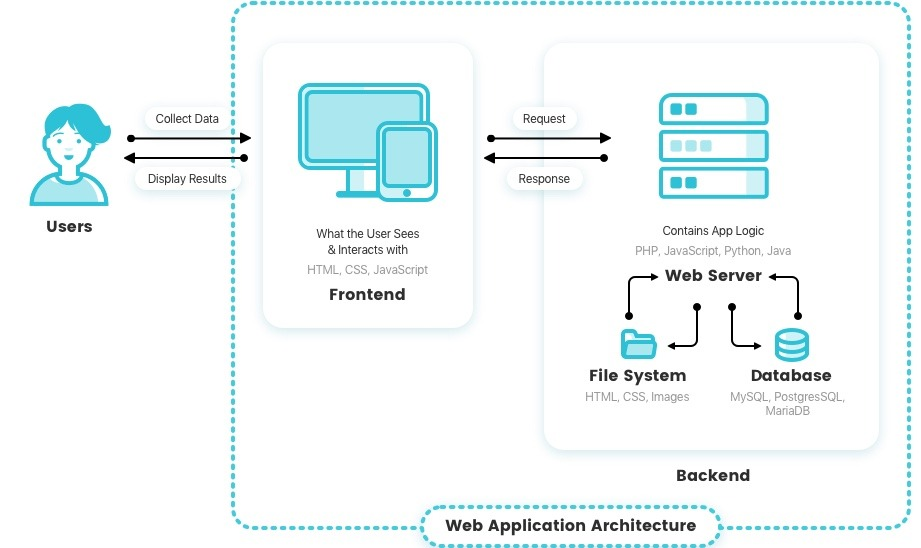
\includegraphics[scale=0.2]{images/architektura}
	\caption{Webes alkalmazás architekúrája}
	\label{abra:Architektura}
\end{figure}

\subsection {A React JavaScript keretrendszer}

Az elmúlt években a React JS jelentős népszerűségre tett szert a webfejlesztés területén. A React egy nyílt forráskódú JavaScript keretrendszer, amelyet a Facebook (Meta) fejlesztett ki, és célja a felhasználói felületek könnyű és hatékony megvalósítása. A React alapvetően egy komponens alapú megközelítést kínál, amely lehetővé teszi a fejlesztők számára, hogy újra felhasználható, önálló építőelemeket hozzanak létre, amelyeket könnyedén kombinálhatnak egymással a komplexebb felhasználói felületek elkészítése érdekében.

A React (\ref{abra:reactLogo}) rendkívül népszerűvé vált a fejlesztők körében számos előnye miatt. Elsőként említhetjük a hatékony Virtual DOM implementációját, amely lehetővé teszi az alkalmazások gyors és hatékony frissítését. A Virtual DOM a weboldal megjelenítéséhez használt valós DOM virtuális reprezentációja. Amikor változás történik az adatokban, a React a Virtual DOM-on keresztül kiszámítja az optimális frissítéseket, majd ezeket a változtatásokat csak a valós DOM-ra alkalmazza. Ez a megközelítés jelentős sebességjavulást eredményez a webalkalmazásokban.

A második fontos előny a komponens alapú megközelítés, amely lehetővé teszi a fejlesztők számára a komponensek újra felhasználását és a kód modularizációját. A React komponensek önmagukban zárt egységek, amelyek különböző feladatokat elláthatnak a felhasználói felületeken, például gombok, űrlapok, listák stb. Az egyedi komponensek könnyedén kombinálhatók egymással, így a fejlesztőknek nem kell újra megírniuk a kódot, hanem egyszerűen felhasználhatják a meglévő komponenseket.

Emellett más technológiai óriások is felfedezték a React előnyeit. Például a Netflix, a PayPal, az Airbnb és a Dropbox is a React-et használja az alkalmazásaik fejlesztéséhez. Ezek a vállalatok magas forgalommal és komplex felhasználói felületekkel rendelkeznek, és a React segítségével könnyedén kezelhetik ezeket a kihívásokat.

Az open-source software (OSS) közösség is hozzájárult a React népszerűségének növekedéséhez. Számos harmadik által (Third party) fél készített könyvtár és eszköz érhető el a React-hez, amelyek további lehetőségeket kínálnak a fejlesztőknek. Ilyen példa a Redux, amely egy állapotkezelő könyvtár, vagy a React Router, amely segít az alkalmazások útvonalainak kezelésében.

A JavaScript önmagában egy típusfüggetlen programozási nyelv, de egyes keretrendszerek, mint a Next.js, a Microsoft által kifejlesztett TypeScript nyelvet használják, amely már megengedi a beépített és személyre szabott típusok használatát.

\begin{figure}[!h]
	\centering
	
\includegraphics[scale=0.04]{images/reactLogo}
	\caption{React logó}
	\label{abra:reactLogo}
\end{figure}

\subsection {A Google Firebase platform}

Mivel a React a webes alkalmazások frontend-jének fejlesztésére szolgál, szükségem volt egy backend szerverre és egy DBMS, -re, amely kiszolgálja a frontend-et, a Google által fejlesztett Firebase platformot és API-kat építettem be az alkalmazásba.
A Google Firebase (\ref{abra:firebaseLogo}) egy teljes körű fejlesztői platform, amely különféle eszközöket és szolgáltatásokat kínál a fejlesztőknek, hogy könnyedén hozzanak létre, teszteljenek és üzemeltessenek webes és mobilalkalmazásokat.

A Firebase Realtime Database egy NoSQL alapú adatbázis, amely valós idejű adatszinkronizációt tesz lehetővé az alkalmazások között. Ez azt jelenti, hogy az adatok automatikusan frissülnek minden csatlakozott eszközön, így a felhasználók valós idejű élményt élvezhetnek. Ez különösen hasznos például csevegőalkalmazások vagy valós idejű játékok fejlesztésekor. 

A Firebase Authentication lehetővé teszi a felhasználók egyszerű és biztonságos hitelesítését. Támogatja az e-mail és jelszó, a szociális média hitelesítés (pl. Google, Facebook, Twitter) és más autentikációs módokat is. A Firebase emellett lehetőséget biztosít a felhasználói fiókok-, profilok kezelésére és jogosultságkezelésre is. 

A Firebase Cloud Storage segítségével könnyedén tárolhatóak és kezelhetőek az alkalmazásban használt fájlok, például képek, hangfájlok vagy videók. Az egyszerű API-k lehetővé teszik a fájlok feltöltését, letöltését és megosztását. Emellett a Firebase Hosting segítségével egyszerűen és gyorsan kiszolgálhatod az alkalmazásod statikus fájljait a világ minden tájáról.

A Storage Bucket-ek egy nagy tárolóhelyet jelentenek a fájlok (például képek, hangfájlok, videók stb.) biztonságos tárolására a felhőben. A Firebase Storage lehetővé teszi a fájlok feltöltését, letöltését, törlését és megosztását egyszerű API-k segítségével. Emellett automatikusan kezeli a fájlok hozzáférési jogosultságait és a CDN révén biztosítja a gyors és megbízható fájlletöltést a felhasználóknak.

\begin{figure}[!h]
	\centering
	
\includegraphics[scale=0.2]{images/firebaseLogo}
	\caption{Firebase logó}
	\label{abra:firebaseLogo}
\end{figure}

\section {Az AES titkosítás}
\subsection {Bevezető}

Az AES egy blokk titkosítási algoritmus, amelyet két belga kriptográfus tervezett 1997-ben. Az algoritmus az 1990-ben meghirdetett nyilvános pályázat nyertese lett, és 2001-ben a NIST (National Institute of Standards and Technology) elfogadta az Egyesült Államok kormányzati szervezetei számára ajánlott titkosítási szabványnak. Mivel az említett pályázat elbírálása publikusan történt, ezért valószínűleg nem történt befolyás a díj megítélését illetően. Az algoritmus egy változata a Rinjdael algoritmusnak, amely eredetileg több blokkmérettel is dolgozott és ebből választották ki az AES-t, amelynek blokkmérete 128 bit.

Az AES blokk mérete 128 bit, és a kulcs mérete lehet 128, 192 vagy 256 bit. Az AES hatékonysága körülbelül 109 Mb/s, amely természetesen függ az adott hardver tulajdonságaitól, és szakértők szerint a 256 bites kulcsméret biztonsága "örök" időkre szól.

Az AES nem használja a Feistel-sémát, mint a DES (Data Encryption Standard), hanem iteratív szerkezetű. Az algoritmus a kulcsméret alapján különböző számú körökben végzi a titkosítást, amelyekhez korkulcsokat generál. A 128 bites kulcs esetén a körök száma 10, a 192 bites kulcs esetén a körök száma 12, míg a 256 bites kulcs esetén a körök száma 14.

Az AES helyettesítést és permutációt alkalmaz a blokkon belül, és véges testek felett végez aritmetikai és műveletet. Az algoritmus térnyerésére az szolgált, hogy a művelet végzés egész számokkal történik, ezért a szerzők egy olyan algoritmust fejlesztettek, ahol az összeadás, kivonás, szorzás, osztás után is halmaz béli elemet kapunk. Az AES véges testként használja a bináris együtthatós polinomokat a GF(2\textasciicircum n) felett, ahol n = 8 fokszámnál kisebb.

Az AES minden műveletet 8 biten végez, és az összes 30 irreducibilis polinom közül a következőt használja: $x\textasciicircum 8 + x\textasciicircum 4 + x\textasciicircum 3 + x + 1$. Az AES minden bájtot a $GF(2\textasciicircum 8) = GF(2)[x]/(x\textasciicircum 8 + x\textasciicircum 4 + x\textasciicircum 3 + x + 1)$ testelemeként kezel.

Az AES-t általában három algoritmus alkotja: a kulcsgenerálás, a titkosítás és a visszafejtés. Az AES a bemeneti 128 bites állapotot (state) egy 4x4-es mátrix formájában kezeli, és az algoritmus minden iterációja során helyettesítő és permutációs műveleteket végez el a blokkon belül.

\subsection {Az algoritmus elmélete}

Az AES a bemeneti adatokat 128 bites blokkokra bontja. A bemeneti adatokat több körön keresztül módosítja míg el nem jutunk a titkosított adatig. A módosításokat az algoritmus több lépésben hajtja végre. Ezeket a lépéseket altranszformációknak nevezzük.

Az altranszformációk három típusúak lehetnek: AddRoundKey, SubBytes és ShiftRows. Az AddRoundKey lépés során az aktuális kör kulcsát XOR művelettel adja hozzá adatblokkhoz. A SubBytes lépés a bemeneti blokk minden elemén végigmegy egy előre meghatározott nemlineáris függvénnyel. A ShiftRows lépés során az adatblokk minden sorát egy bizonyos számmal rotáljuk.

Összességében az AES titkosítási algoritmus magában foglalja a bemeneti adatok blokkokra bontását, majd a bemeneti blokkokon végrehajtja az altranszformációkat több körön keresztül, amíg meg nem kapja a titkosított adatot. Az algoritmus célja az adatok biztonságos és hatékony titkosítása a megfelelő védelem érdekében.

\subsection {Az algoritmus gyakorlatban}

Az alábbi kódrészlet az AES algoritmus egyik használati módja JavaScript programozási nyelven a CryptoJS könyvtárcsomag segítségével (\ref{code:encryption}).

\begin{lstlisting}[caption={Titkosítás példakód.}, captionpos=b, language = JavaScript, label={code:encryption}]
export const encryptData = text => {
  const salt = CryptoJS.lib.WordArray.random(128 / 8);
  const key = CryptoJS.PBKDF2(secretPass, salt, {
    keySize: 256 / 32,
    iterations: 1000,
  });
  const iv = CryptoJS.lib.WordArray.random(128 / 8);

  const encrypted = CryptoJS.AES.encrypt(JSON.stringify(text), key, {
    iv: iv,
    mode: CryptoJS.mode.CBC,
    padding: CryptoJS.pad.Pkcs7,
    tag: true,
  });

  const data = {
    ciphertext: encrypted.ciphertext.toString(CryptoJS.enc.Base64),
    iv: iv.toString(CryptoJS.enc.Base64),
    salt: salt.toString(CryptoJS.enc.Base64),
    tag: true,
  };
  return JSON.stringify(data);
};
\end{lstlisting}

A kód első lépése a \textit{salt (só)} generálása, ami egy 128/8 bájt szekvencia, amely segítségével meghatározásra kerül majd a key (kulcs). A \textit{CryptoJS.lib.WordArray.random(128 / 8)} kódsor a \textbf{CryptoJS} könyvtárban található \textit{random()} függvény hívásával egy véletlenszerű 128-bites szekvenciát generál, majd beilleszti az adatokat a WordArray osztályba.

A következő lépésben a kulcs előállítása történik meg a \textit{secretPass (jelszó)} és a só használatával a kulcsderiváló függvény segítségével. A kulcs előállítása a \textit{CryptoJS.PBKDF2()} függvénnyel történik, amely egy kulcstervező függvény. Az első paraméter a titkosításhoz használt jelszó, a második argumentum a só, a harmadik pedig a kulcs hosszát és az iterációk számát határozza meg. Ennél az algoritmusnál nagyon fontos odafigyelni, hogy a jelszó szigorúan titkos információ, vagyis ezt biztonságosan ajánlott eltárolni szerver oldalon. A többi paraméter publikus, mert önmagukban nem elegendőek a titkosított szöveg visszafejtéséhez.

Az inicializáló \textit{vektor (iv)} generálása következik. Az IV egy véletlenszerű bájt szekvencia, amelynek hossza megegyezik a blokk méretével (128 bit), és a titkosítás során használják, hogy azonos adatok esetén is véletlenszerű kimenetet generáljon.

Az adat titkosítása a \textit{CryptoJS.AES.encrypt()} függvénnyel történik. Az adatot először JSON formátumba alakítjuk, majd az AES algoritmust a kulcs, az IV és további paraméterek (mód, padding és tag) megadásával alkalmazzuk. A \textit{mode} a blokktitkosítási mód (BCM) kiválasztására szolgál, ezek között található a ECB, CBC, OFB vagy CFB. A mi esetünkben a CBC (Cipher Block Chaining) mód van használva.

A  \textit{padding} a blokkok kitöltési módját határozza meg, itt a \textbf{Pkcs7} (Public Key Cryptography Standards 7-es szabványa) van használva. A Pkcs7 padding szabvány szerint, ha az üzenet hossza nem egész blokk méretű, akkor azt szükséges kiegészíteni. Minden hiányzó bájt felveszi a hiányzó bájtok számának megfelelő értéket. Ha például az utolsó blokkban 3 hiányzó bájl van, akkor a blokk utolsó bájtjai a 0x03 értéket vesz fel.

Az textit{iv} az inicializáló vektort tartalmazza, amit korábban generáltunk. A textit{tag} beállítása igazra van állítva, hogy az üzenet hitelesítése (integritásának ellenőrzése) is megtörténjen a titkosítás során. A tag az üzenet elejére kerül beillesztésre a titkosítás során, és végül az eredeti üzenet végén kerül ellenőrzésre a helyessége.

Az utolsó lépés a textit{titkosított adat (ciphertext)}, az IV, a só és az üzenet hitelesítésének értéke (tag) összekapcsolása és JSON formátumba rendezése és visszatérítése.

\pagebreak
Az alábbi példakód a visszafejtést valósítja meg (\ref{code:decryption}):

\begin{lstlisting}[caption={Visszafejtés példakód.}, captionpos=b, language = JavaScript, label={code:decryption}]
export const encryptData = text => {
  const salt = CryptoJS.lib.WordArray.random(128 / 8);
  const key = CryptoJS.PBKDF2(secretPass, salt, {
    keySize: 256 / 32,
    iterations: 1000,
  });
  const iv = CryptoJS.lib.WordArray.random(128 / 8);

  const encrypted = CryptoJS.AES.encrypt(JSON.stringify(text), key, {
    iv: iv,
    mode: CryptoJS.mode.CBC,
    padding: CryptoJS.pad.Pkcs7,
    tag: true,
  });

  const data = {
    ciphertext: encrypted.ciphertext.toString(CryptoJS.enc.Base64),
    iv: iv.toString(CryptoJS.enc.Base64),
    salt: salt.toString(CryptoJS.enc.Base64),
    tag: true,
  };
  return JSON.stringify(data);
};
\end{lstlisting}

A \textbf{decrypt} függvény az \textbf{encrypt} függvénnyel ellentétes sorrendben dolgozza fel az adatokat. A paraméterként kapott titkosított szövegből JSON objektumot állít elő. Ezután ebből az objektumból megkapja a só és az iv Base64 formátumból az értékeket. A kulcs előállítása a \textit{PBKDF2} függvénnyel történik a jelszó és a só segítségével. A titkosított adat, az iv, a só és a hitelesítési tag felhasználásával sikeresen vissza tudjuk fejteni az eredeti üzenetet.

\subsection{Alkalmazások és érdekességek}

\begin{itemize}
	\item Az AES algoritmusnak 128, 192 és 256 bites változatai vannak, amelyek mindegyike különböző szintű biztonságot nyújt.
	\item Az algoritmus rendkívül hatékony, amely lehetővé teszi a titkosított adatok nagy sebességű feldolgozását.
	\item Nyilvánosan elérhető és ingyenesen használható, ami azt jelenti, hogy bárki használhatja és integrálhatja az alkalmazásába.
	\item Ennek az algoritmusnak számos könyvtárcsomagban van megvalósítva. Léteznek egyaránt publikus és privát forráskódok, amelyek közül néhány optimalizálva van a hardveres és szoftveres rendszerekhez.
	\item Az alkalmazása különböző területeken népszerű, például az online banki- és pénzügyi tranzakciókban, a VPN (Virtual Private Network) rendszerekben, a Wi-Fi hálózatokban, az adattároló eszközökön.
	\item Az AES használata akkor biztosít teljes biztonságot, ha ezt együtt használják egyéb kriptográfiai primitívekkel. Ilyen az AES-en kívül az RSA vagy a Hashmap. A kulcsfontosságú védelmi rendszerekben, mint például a HTTPS, SSH vagy TLS, használnak több rétegű védelmi mechanizmusokat az AES kiegészítéseként.
	\item A 256 bites titkosítási kulcsokat sokkal nehezebb brute-force módon támadni, mint egy 128 bites kulcsot. Azonban az utóbbi is olyan hosszú időbe telik kitalálni, még hatalmas számítási kapacitás mellett is, hogy az előrelátható jövőben nem lesz probléma, mert egy támadónak is hatalmas számítási kapacitásra lenne szüksége a szükséges brute-force (nyers-erő módszere) generáláshoz.
	\item Azonban a 256 bites kulcsokhoz is több feldolgozási teljesítmény szükséges és hosszabb ideig tarthat a generálásuk. Amikor az energiafogyasztás problémát jelent, különösen kis eszközök esetében, vagy a késleltetés valószínű, a 128 bites kulcsok jobb választásnak számítanak.
\end{itemize}

\section {RSA!!!!}

\section {Kutatási kérdések}

Az alkalmazás fejlesztése során a következő kérdésekre próbáltam válaszokat keresni:
\begin{itemize}
	\item Hogyan lehet biztonságosabbá tenni az elektronikus jegyvásárlást és azok felhasználását?
	\item Mely technológiák segítségével lehet gyors és hatékony online üzletet tervezni és megvalósítani?
	\item Hogyan lehet a megvalósított rendszert hosszú távon karban tartani és felügyelni?
	\item Hogyan lehetséges a rendszer automatizálása valós időben?
\end{itemize}

\section {Célkitűzések}

A kutatási kérdésekre keresett válaszok során felmerültek további kérdések, amelyek hozzájárulnak a céljaim pontosabb megfogalmazásában:
\begin{itemize}
	\item Hol és hogyan fogom tárolni a felhasználói- és alkalmazás adatokat?
	\item Hogyan fogom kelelni a felhasználói jogosultságokat, hogy minden felhaszáló csak a saját adataihoz férjen hozzá?
	\item Hogyan fogom megvalósítani a többlépcsős azonosítást a jegyek felhasználásásnál?
	\item Hogyan fogom eljuttatni a felhasználóknak a megvásárolt termék(ek)ről és azok azonosításához szükséges információkat? 
	\item Hogyan tudom a felületet felhasználó baráttá tenni?
\end{itemize}

A megfogalmazott kérdések azt a legfontosabb célt hivatottak szolgálni, hogy egy kényelmes és megbízható alkalmazás jöjjön létre a felhasználók számára. Ennek megvalósításához szükséges szempont, hogy megbizonyosodjanak a felhasználók, hogy a felület használata nem félreérthető és nincsenek olyan működési aspektusok, amelyek zavarhatják a felhasználói élményt.

Az előbbiek elérésére a kisebb célok egy még pontosabb képet tudnak biztosítani számomra, hogy megfelelő ütemben haladjon a fejlesztés anélkül. hogy kimaradjanak fontos részletek.

A fent felsorolt kérdések felhívják a figyelmet arra a fontos tényezőre, hogy az egyre elterjedtebb körű internet használatának korszakában elengedhetetlen a felhasználók személyes adatainak a védelme. Ennek megvalósítására is érdemes számos megoldást kutatni és majd kiválasztani az alkalmazás szempontjából megfelelőt.

Továbbá a előzőek mellett megoldást kell kapjak arra a problémára, hogy a jelenleg is működő oldalak nagy része nem foglalkozik azzal a tényezővel, hogy egy elektronikus jegy nagyon sok veszélynek van kitéve és ennek ellenére nem alkalmaznak többlépcsős azonosítást a jegyek hitelesítésekor. Ennek egyszerűen az az oka, hogy bizonyos százalékban lassítaná a hitelesítési folyamatot és az eladók nem vállalnak felelősséget a jegyek esetleges elveszítése vagy ellopása esetén.

Végül de nem utolsó sorban fontos, hogy lehetőséget biztosítsak az alkalmazás viselkedésének monitorizálására, valamint az alkalmazás továbbfejleszthetőségére. Az alkalmazás működésének megfigyelése során olyan hibákról és ötletekre kaphatok visszajelzést, amivel tudom biztosítani az alkalmazás hosszútávú karbantartása és továbbfejlesztése érdekében.